\documentclass[article,12pt,twocolumn]{IEEEtran}
\usepackage[utf8]{inputenc}
\usepackage{amsmath}
\usepackage{graphicx}
\usepackage{gensymb}

\title{Assignment Q8 b}
\author{Suryaansh Jain}
\date{March 2022}

\begin{document}

\maketitle


$
\begin{array}{l}
\angle B A Q=30^{\circ}\\
\Rightarrow \angle B A C=30^{\circ}\\
\text { also\  } \angle C A P=180^{\circ}-\angle C A Q \Rightarrow \angle C A P=120^{\circ}\\
\Rightarrow \angle C A D=\angle P A D=60^{\circ}\\
\Rightarrow \angle B A D=90^{\circ}\\
\Rightarrow B D \text {\ is\ a\ diameter }\\
\angle A D B=\angle A C B=30^{\circ} \text {\ [Angle\ made\ a\ chord\ at\ two\ different\ points\ ]}\\
\text {also\ } \angle C A B=30^{\circ}\\
\Rightarrow \triangle A B C \text {\ is\ an\ isosceles \ triangle }
\end{array}
$

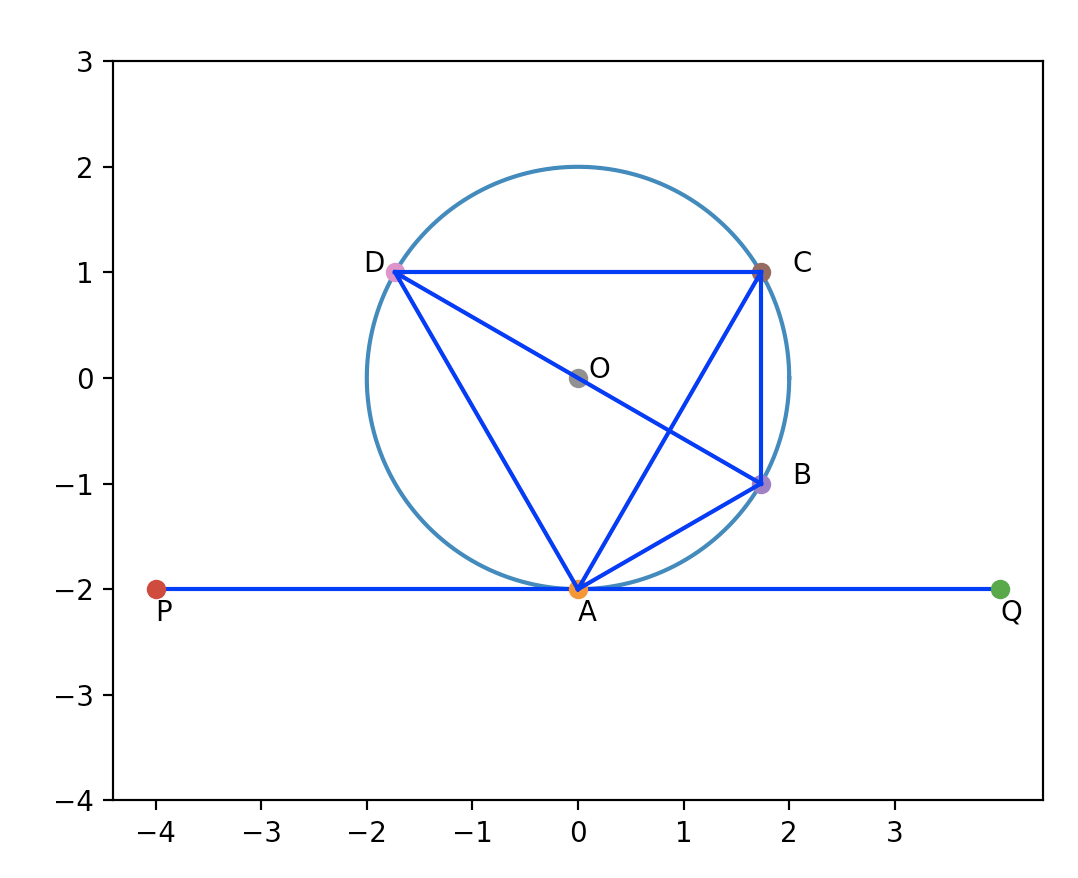
\includegraphics[scale = 0.4]{output.png}

\end{document}
